\newpage
\section{Durchführung}
\label{sec:Durchfuehrung}

\subsection{Die Feder}
\label{sec:feder}
Verwendet wird eine Trompetenfeder, welche in der Möbelbeschlagindustrie in Schubladeneinzugsystemen
verwendet wird \ref{fig:schublade}. 
Der Federtyp zeichnet sich durch die nicht klassische Ösenform aus, welche die Problematik des Ösenbruchs umgeht.\\

Wichtig ist anzumerken, dass die Ruhelänge $L_0$ in der Praxis lediglich als anzustreben gilt.
Die Länge der Zugfeder vergrößert sich bei Belastung, deshalb bedarf es keiner festgeschrieben Maximallänge für $L_0$, da
der Einbauraum stehts auf eine großerwerdene Feder ausgelegt ist.  

\begin{center}
    \makebox[\textwidth]{
        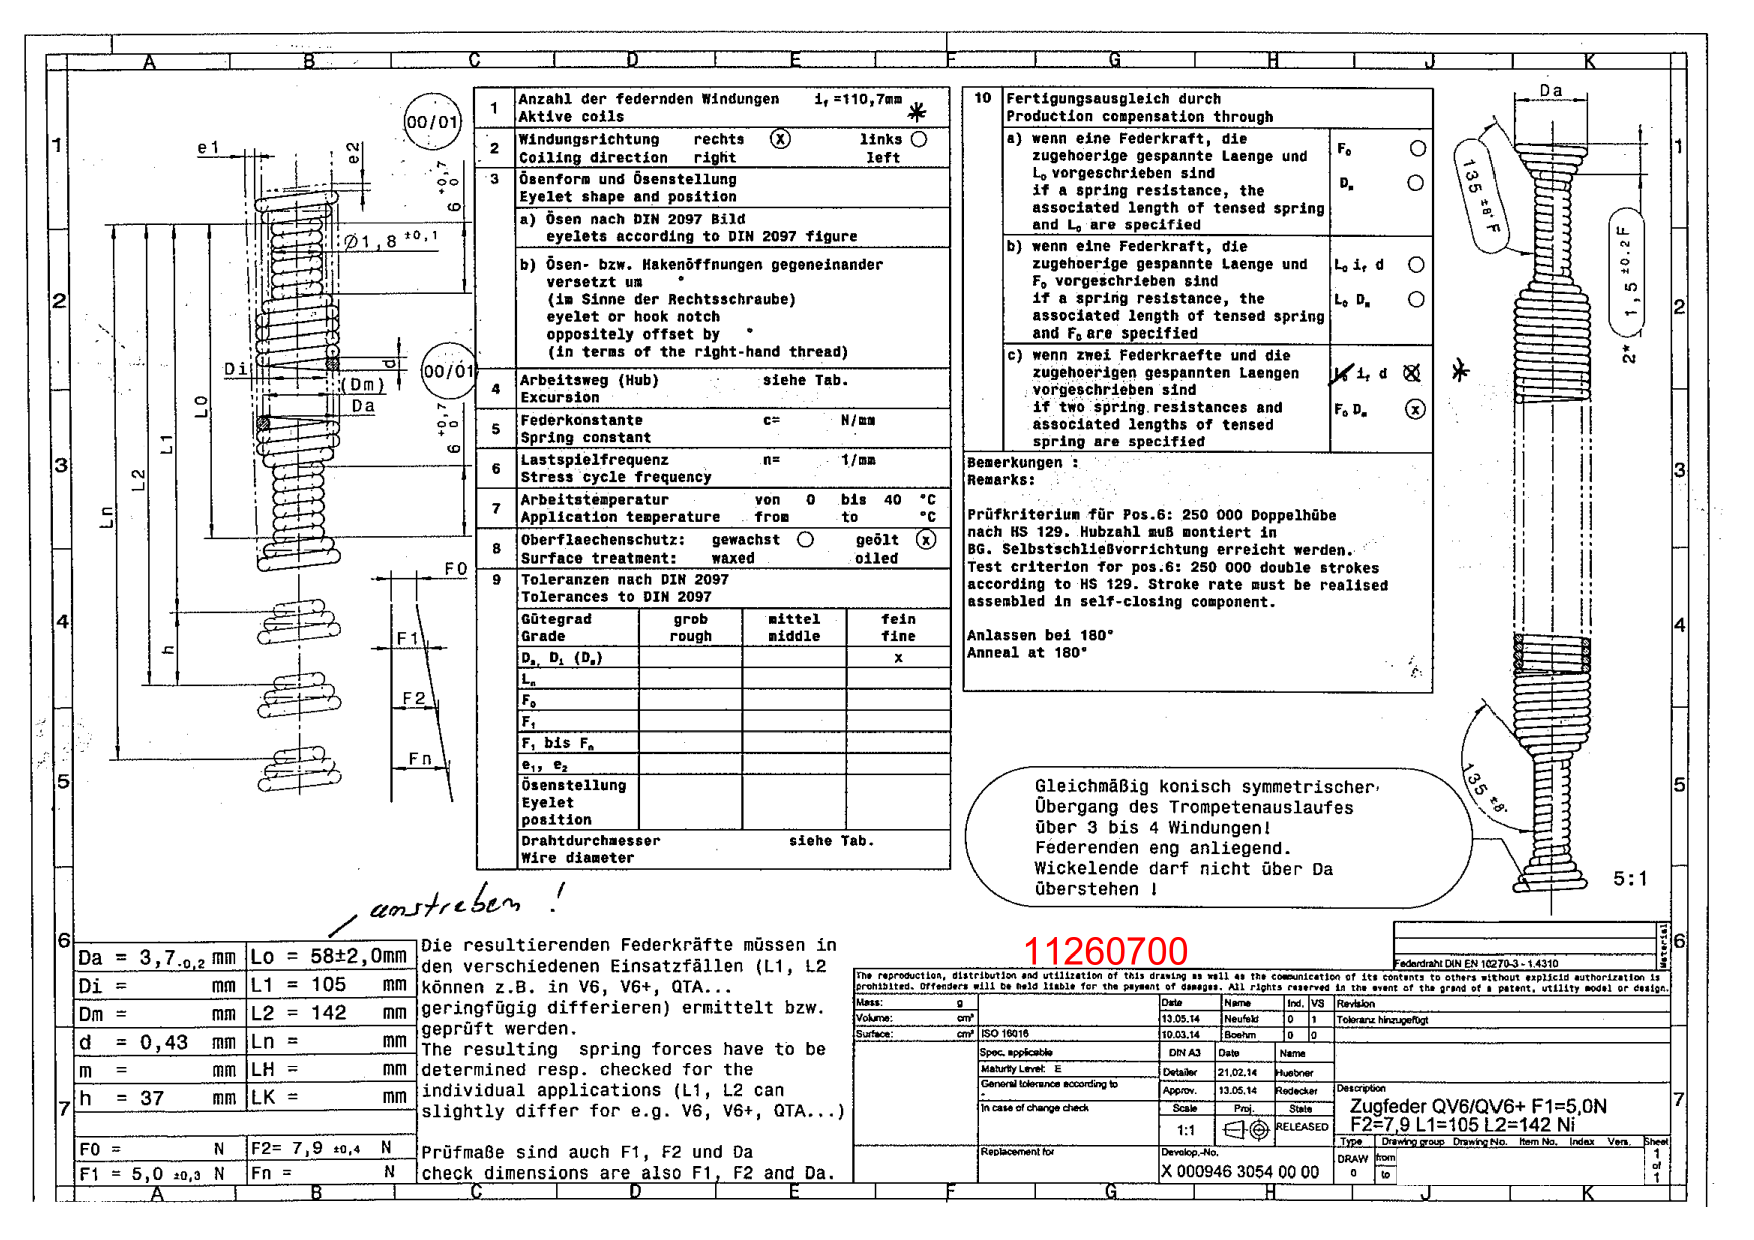
\includegraphics[width=\paperwidth]{bilder/zeichnung_11260700.pdf}
        \label{fig:zeichnung}
        }
\end{center}
Im Folgenden kann die Feder als zylindrische Feder betrachtet werden,
da die Belastung in der Größenordung liegt, sodass der zu federnde Anteil nicht 
vom Trompentenanteil (gemeint sind hier die Ösenteile am Ende der Feder)
ausgeführt wird, da bei der Kraftprüfung die größte zulässige Prüflänge $Ln$ mit 
$Ln>L2$ nicht überschritten wird.\\
Die nach der Zeichnung gefertigten Feder wird im folgenden Basisfeder genannt.
\label{subsec:feder}
\subsection{Vorgehen}
Folgendes wird untersucht:
\begin{enumerate}
    \item   Die Basisfeder wird in einer Stückzahl von 6 anhand der Zeichnung produziert.\\
            Gemessen wird jeweils der Federaußendurchmesser $D_a$ und die Federlänge 
            $L0$ und die Gesamtmasse $m$ der 6 Federn sowie die Kräfte $F1$ und $F2$ an $L1$ und $L2$ mithilfe eines Newtonkraftmesser aus Abb. \ref{fig:kraftmesser}.
            Dort können die Federn gespannt werden und auf die zuprüfenden Längen gestreckt werden.\\
            Anschließend werden die Werte $D_a$, $L0$, $F1$ und $F2$ gemittelt (Feder 1).

    \item   Nun wird der Federaußendruchmesser $D_a$ um ca. $\pm0.1$mm varriert und in einer 
            Stückzahl von jeweils 5 produziert.\\
            Die Federn werden an $D_a$, $L0$, $m$, $F1$ und $F2$ vermessen und gemittelt (Feder 2, Feder 3).\\
            Die gemittelte Federn (Feder 1,2,3) werden in einem Kraft-Weg-Diagramm eingetragen und
            die Federraten $R$ über die Steigung einer Ausgleichsgeraden, sowie die Vorspannkraft $F0$ 
            über den y-Achsenabschnitt bestimmt.\\
            Anschließend wird der Einfluss der Federdicke $D$ auf die Federkonstante $R$ ermittelt
            und nach Gl. \ref{eqn:federrate} $R \propto D^{-3}$ gefittet und mit der Theoriekurve verglichen.

    \item   Nun wird die Windungszahl $n$ um ca. $\pm 10$ Windungen varriert und in einer Stückzahl von 5 produziert.(Feder 4, Feder 5)\\
            Es wird analog zu 2 vermessen und gemittelt und ein Kraft-Weg-Diagramm erstellt und
            daraus $R$ und $F0$ aus einer Ausgleichgeraden ermittelt und mit der Theoriekurve verglichen.
            Anschließend wird der Einfluss der wirkenden Wicklungszahl $n_{wirk}$ auf die Federkonstante $R$ ermittelt
            und nach Gl. \ref{eqn:federrate} $R \propto n_{wirk}^{-1}$ gefittet und mit der Theoriekurve verglichen.

    \item   Nachfolgend soll die Massenentwicklung in Bezug auf die veränderten Paramter untersucht werden.
    Dazu wird zunächst die Federmasse $m$ in  Abhängigkeit der Federrate $R$ aufgetragen. Anschließend
    wird die Massenentwicklung $m$ aufgrund der Veränderung im mittleren Federdurchmesser $D$ und Wicklungszhal $n$
    näher betrachtet.
\end{enumerate}
\begin{figure}[H]
    \centering
    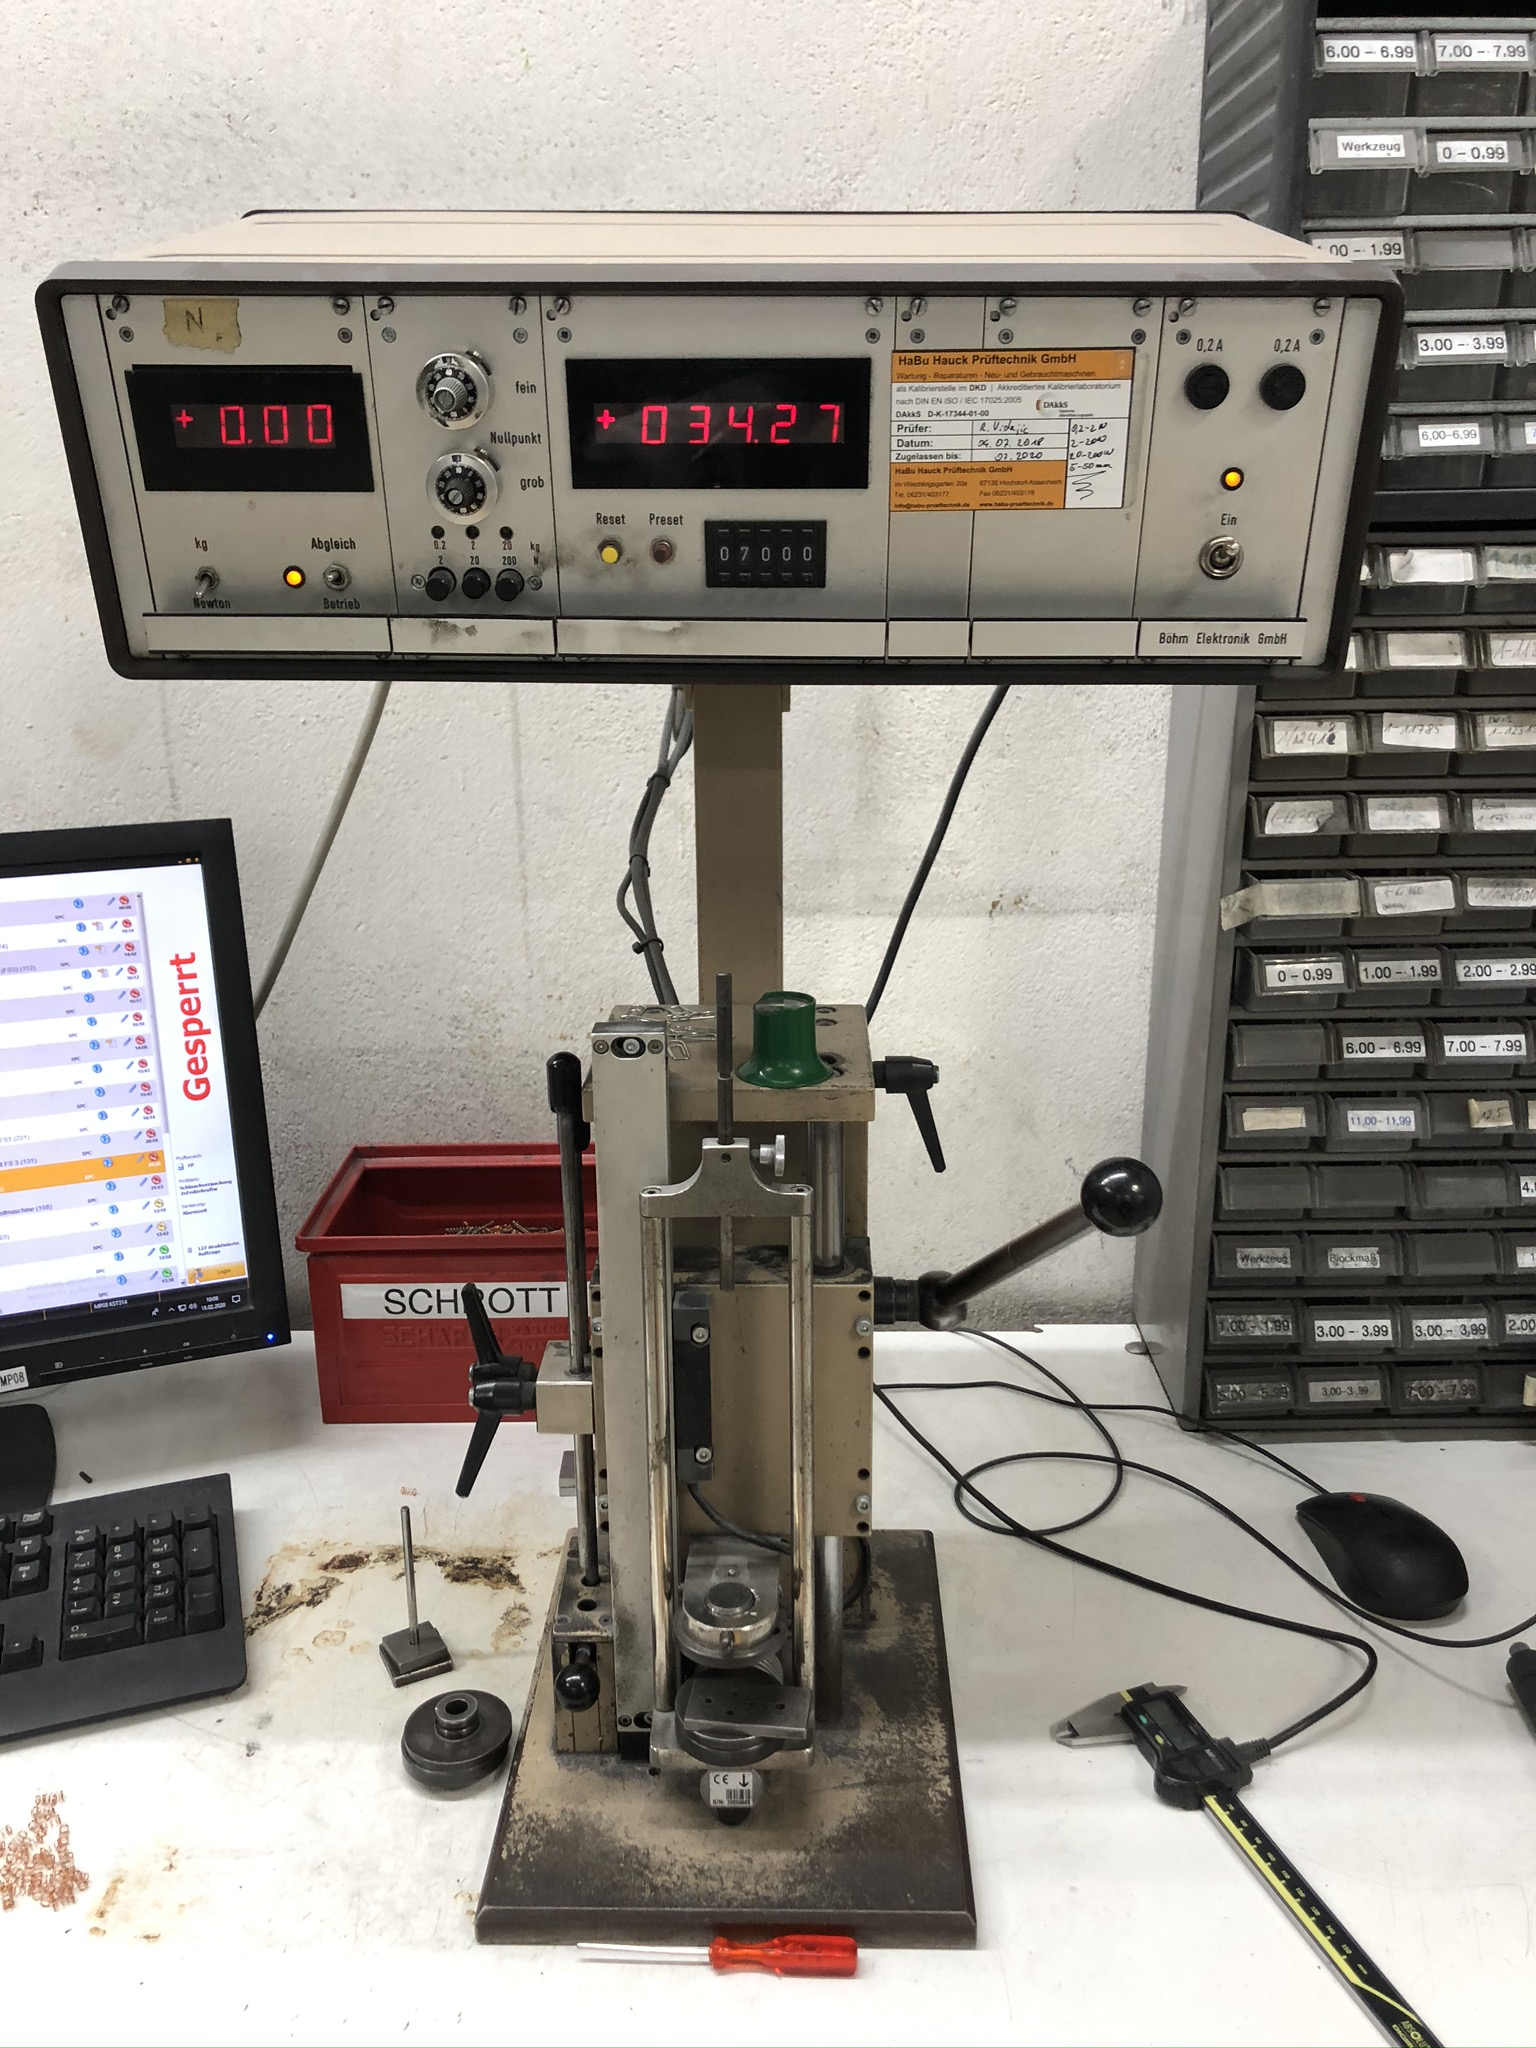
\includegraphics[width=0.5\textwidth]{bilder/fotos/kraftmesser.JPEG}
    \caption{Der Newtonkraftmesser lässt sich auf zwei spezifische Federwege (hier: L1 und L2)
    einstellen. Die Feder wird eingespannt und über einen Hebel beansprucht. Über die digitale Anzeige
    lässt sich die wirkende Kraft (hier dann F1 und F2) ablesen.}
    \label{fig:kraftmesser}
\end{figure}
\begin{figure}[H]
        \centering
        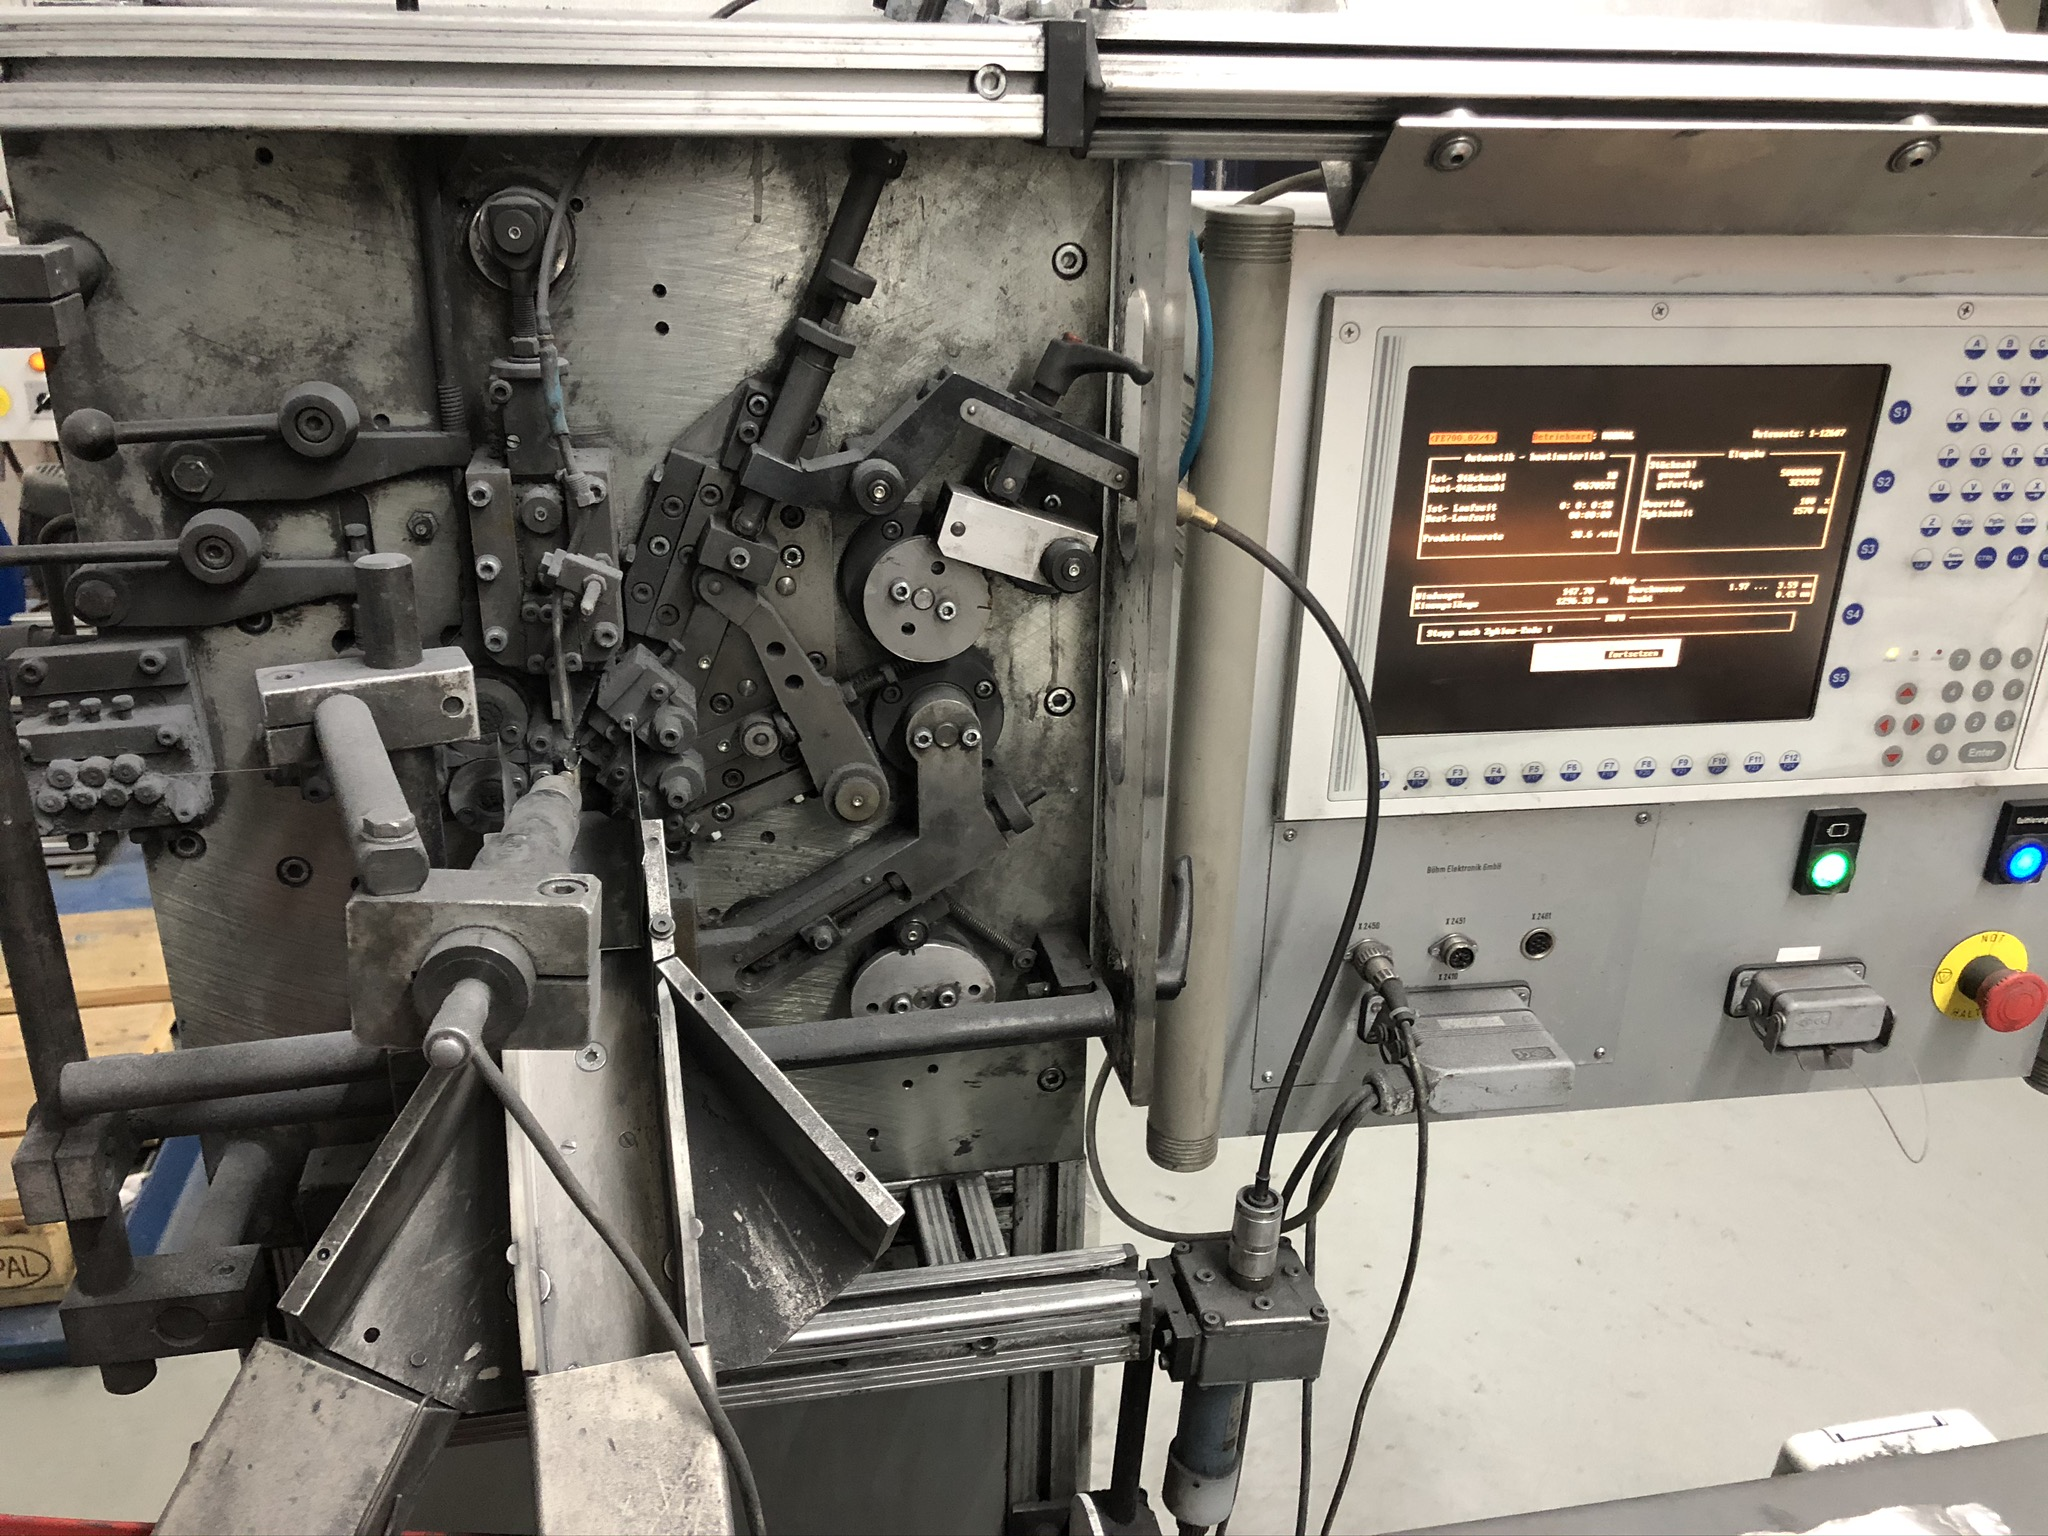
\includegraphics[width=0.5\textwidth]{bilder/fotos/maschine_gesamt.JPEG}
        \caption{Federwindeautomat NC-4Achsen-Maschine}
\end{figure}
\begin{figure}[H]
        \centering
        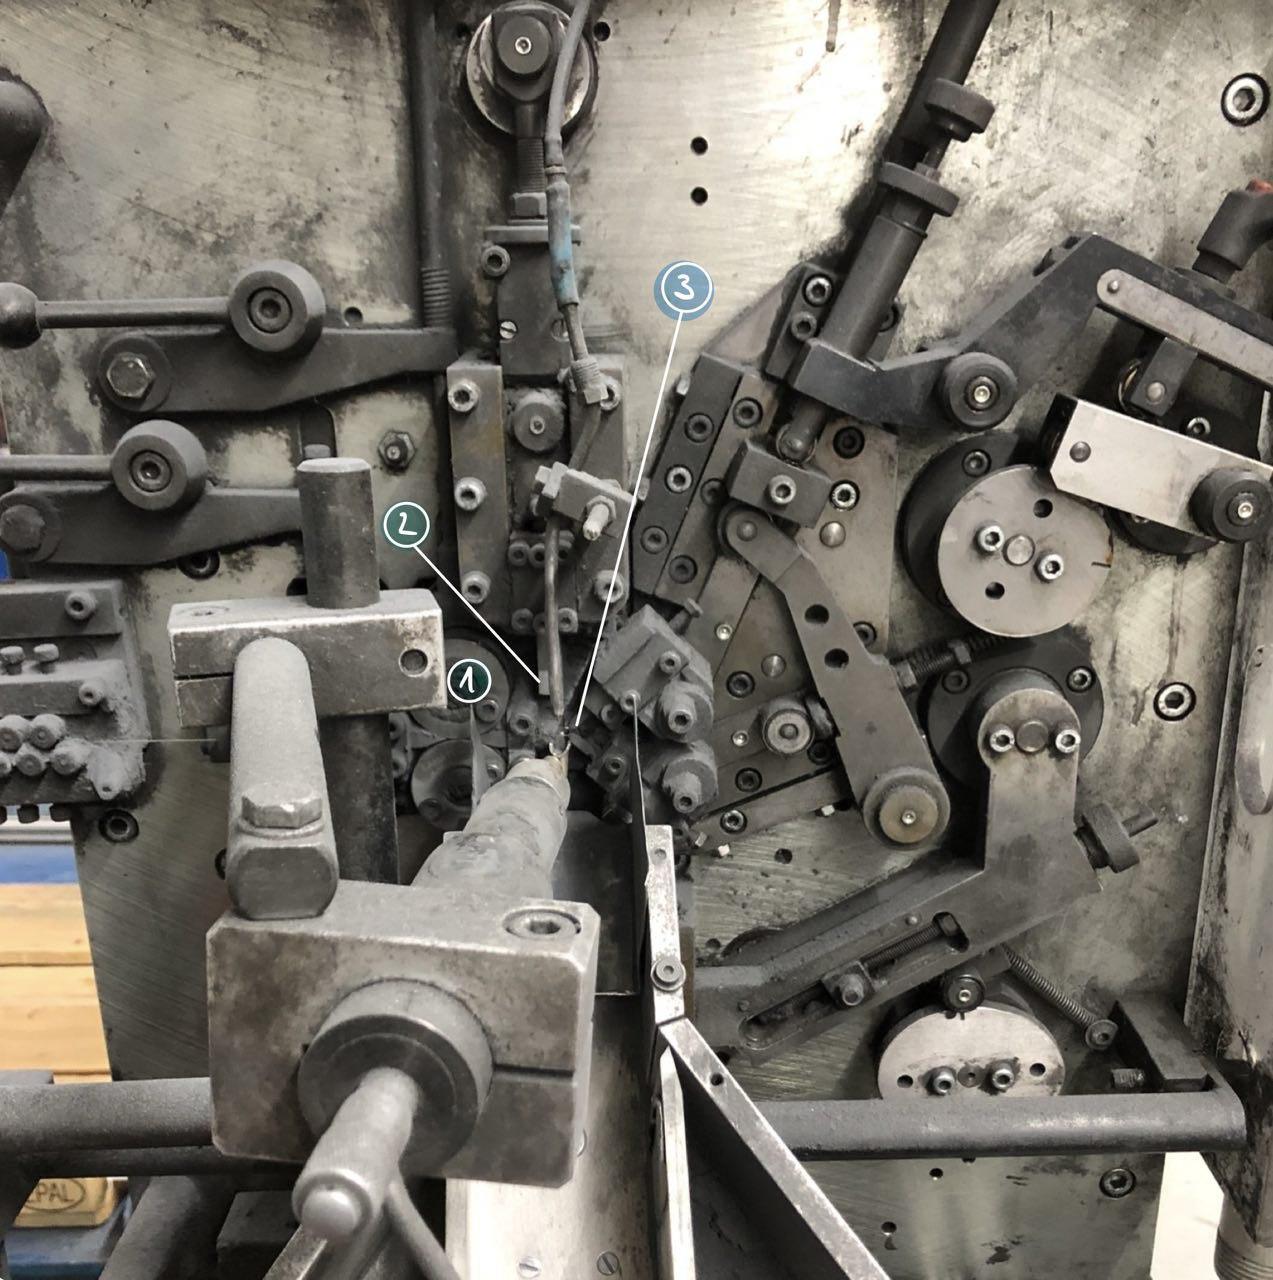
\includegraphics[width=0.5\textwidth]{bilder/fotos/maschine_nah_beschriftet.jpg}
        \caption{NC-4Achsen-Maschine Federwindeautomat.\\
        1)Einzugswalze\\
        2)Abschneidmesser\\
        3)Wickelstift}
\end{figure}

\begin{figure}[H]
        \centering
        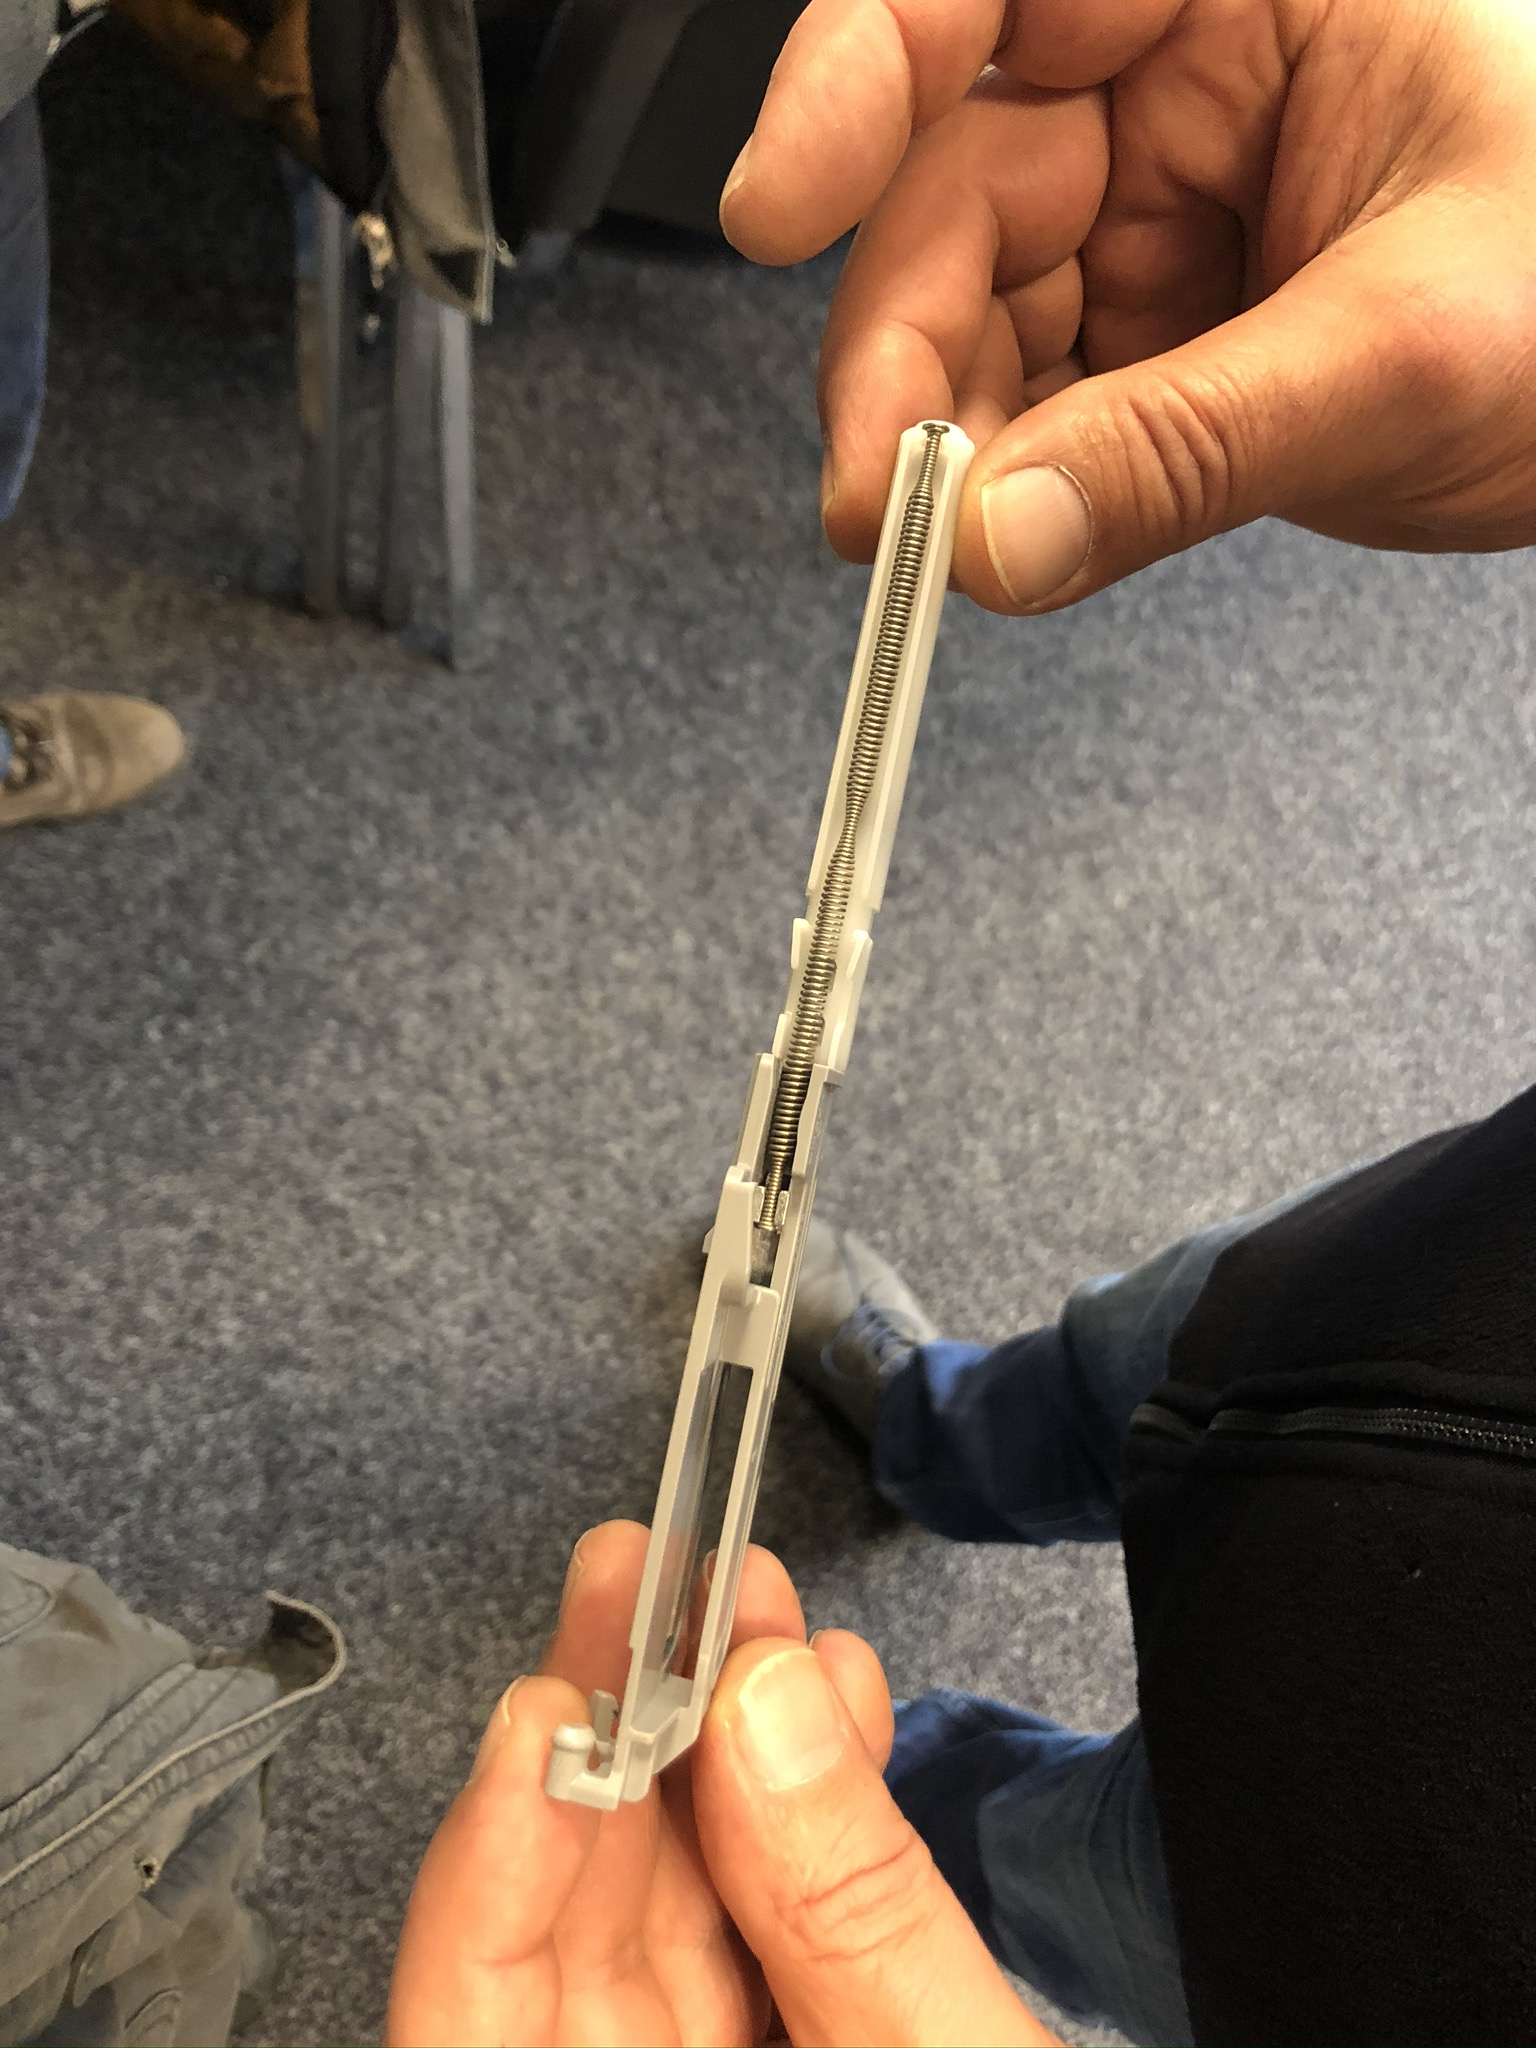
\includegraphics[width=0.5\textwidth]{bilder/fotos/schublade.JPEG}
        \caption{Späteres Einbauteil. Ein Schubladeneinzugsystemen für Möbel.}
        \label{fig:schublade}
\end{figure}